%!TEX root = ../doc.tex
\chapter{Ist Analyse}
\label{sec:istanalyse}
\section{Imagin Cargo}
Imagine Cargo operiert im DACH-Raum (Deutschland, Österreich und Schweiz) und bietet die nachhaltige Expresskurier-Dienstleistung in 15 Städten an. Das Startup wurde 2014 von Nick Blake und David Emmerth gegründet und beschäftigt zur Zeit XY Mitarbeiter. Für das Unternehmen wurde ein Business Model Canvas erstellt, welches in der Abbildung \ref{fig1:businessmodelcanvas} zu sehen ist. Business Model Canvas sind Vorlagen um neue Prozesse zu entwickeln bzw. bestehende Prozesse zu dokumentieren.
\begin{figure}[ht]
	\centering
  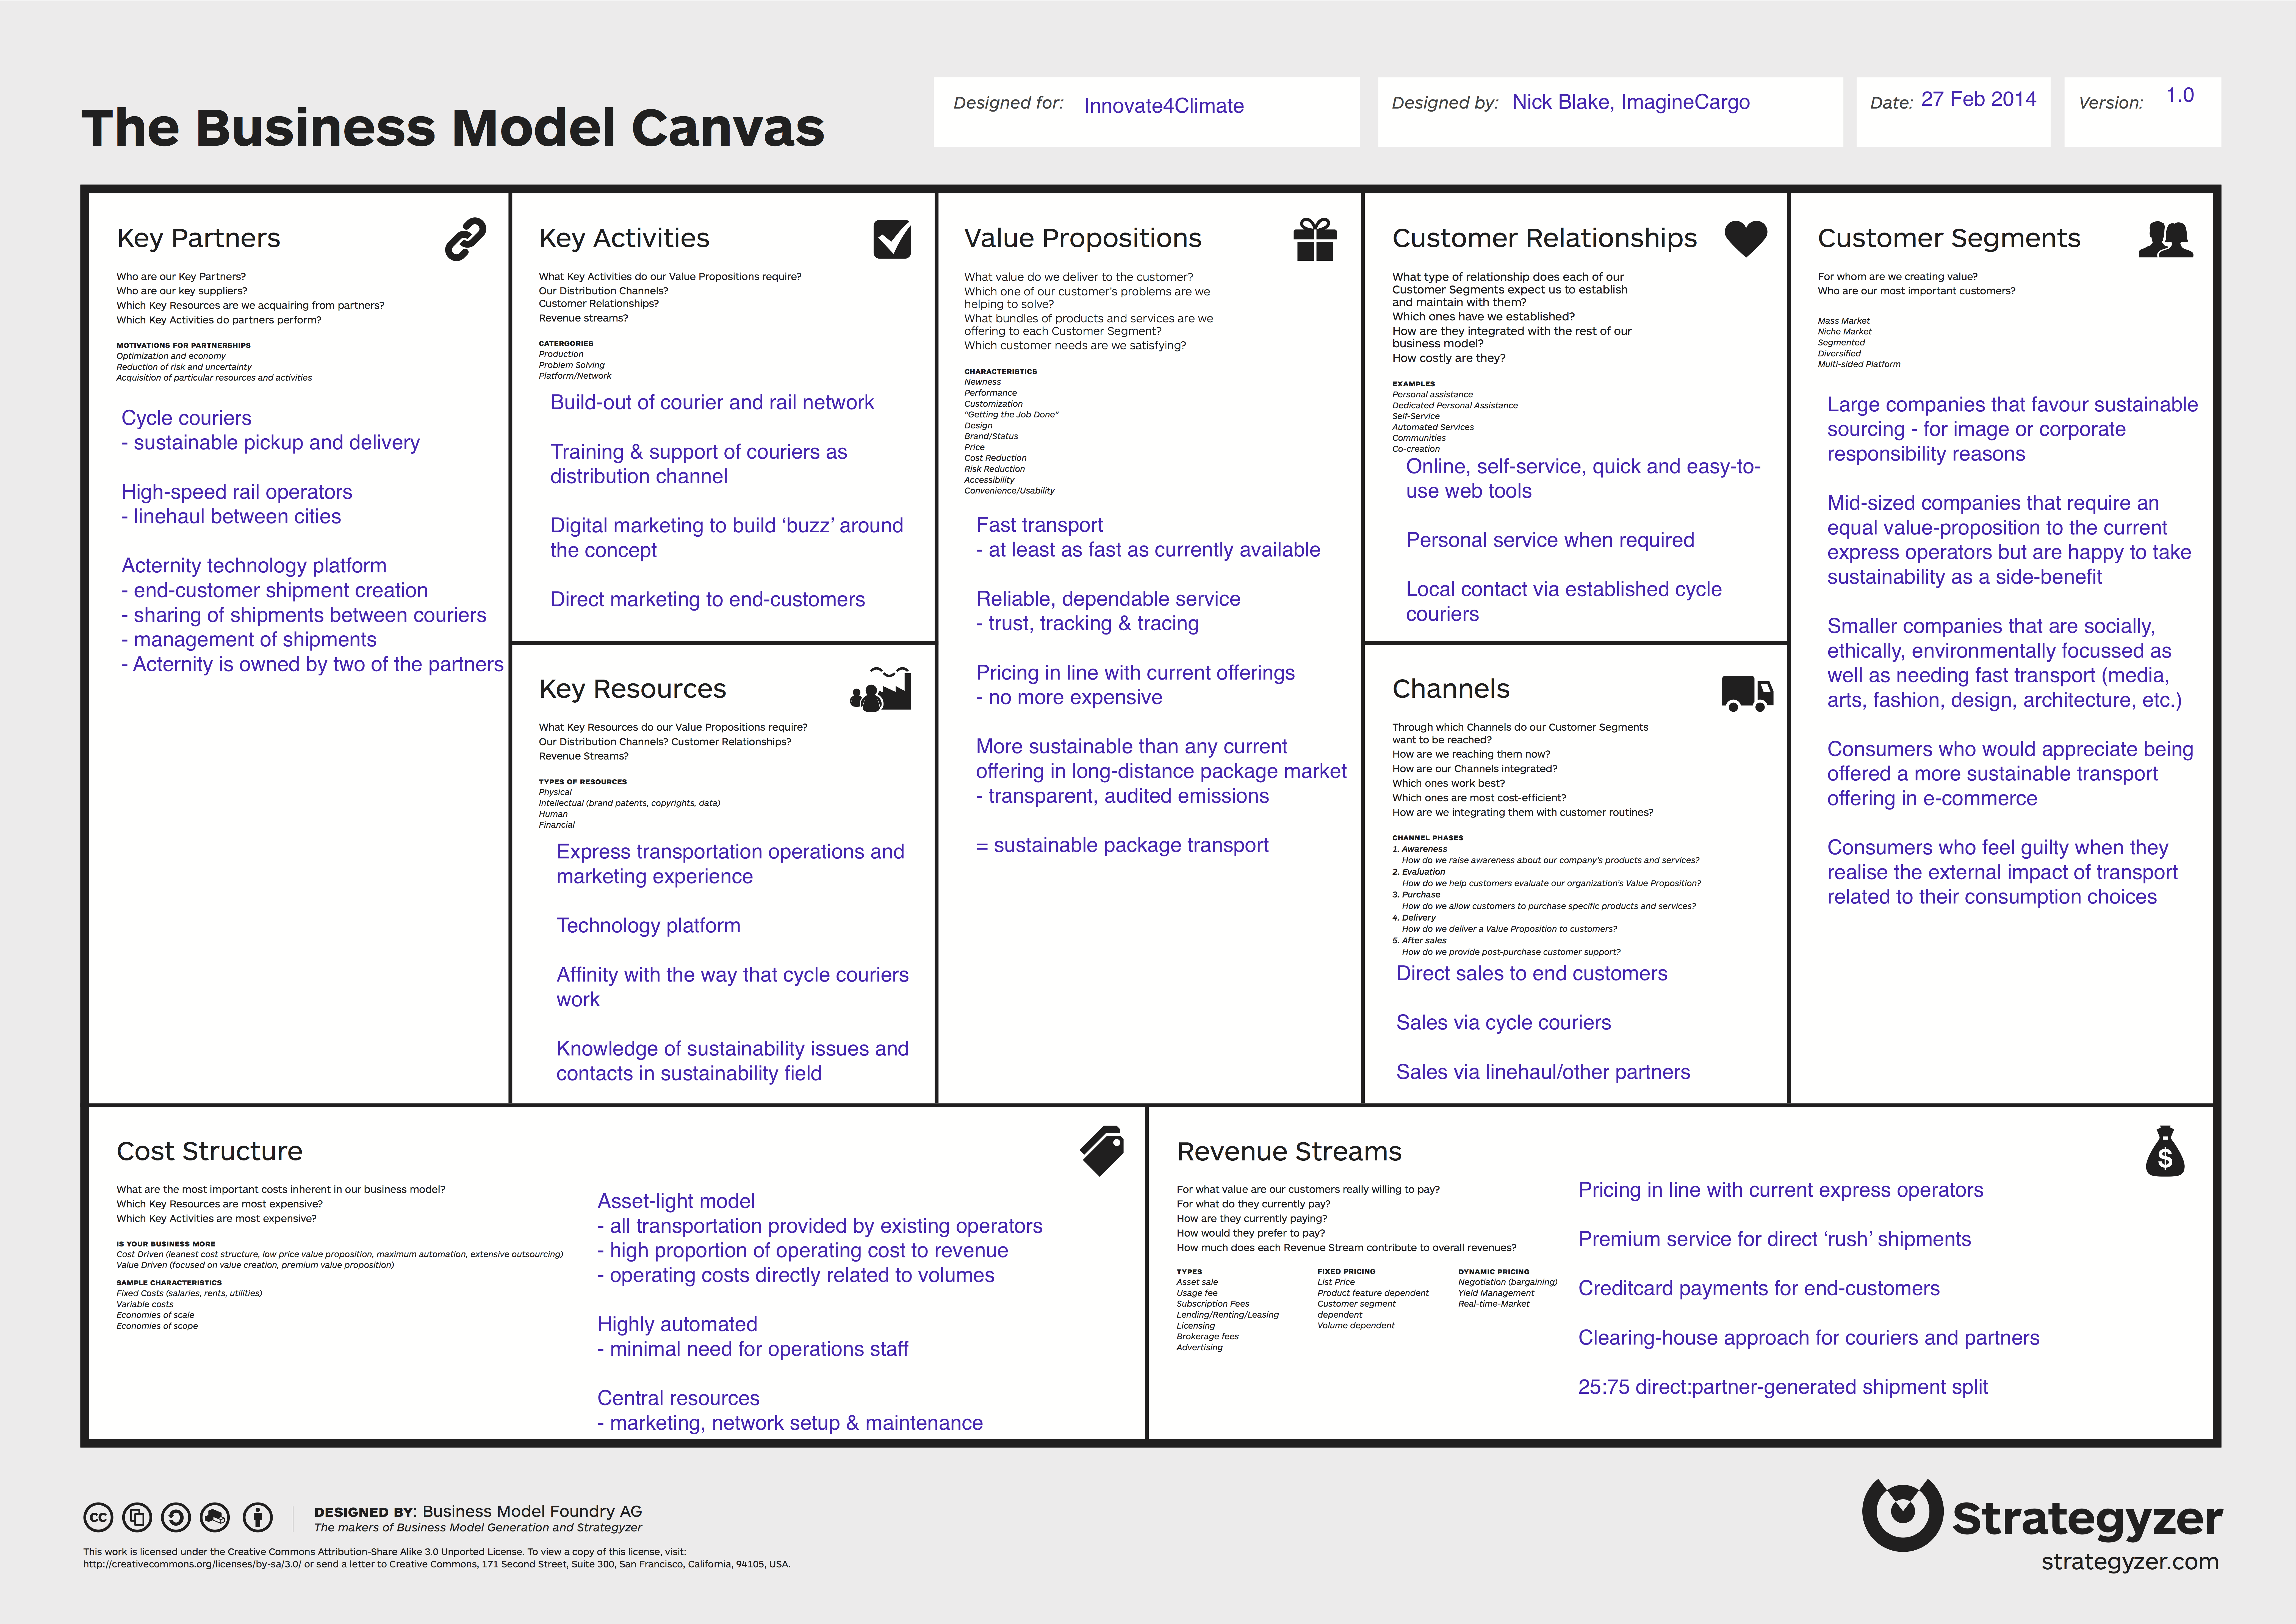
\includegraphics[width=0.88\textwidth]{images/businessModelCanvas.png}
	\caption{Business Model Canvas von Imagine Cargo}
	\label{fig1:businessmodelcanvas}
\end{figure}
 Die Mitarbeiter von Imagine Cargo haben rotierend die Rolle des Disponenten, welcher Aufträge per Mail oder Telefon annimmt und alle notwendigen Schritte für eine erfolgreiche Lieferung ausführt. Auf der Webseite von Imagine Cargo exisitiert eine \textit{wufoo-Form} mit welchem über HTML 5 Form Elemente die benötigten Informationen eingegeben werden können und danach per Mail an den Zuständigen Disponenten geschickt werden. Der Prozess wird im Kapitel \ref{subsec:prozess} genauer beschrieben.

--> Einschub Deutschland problematik mit lieferung.


\subsection{Prozesse}
\label{subsec:prozess}
LoBo wurde ursprünglich für die Verwaltung und Koordinierung von Fahrradkurieren in \textbf{einer} Stadt entwickelt. In LoBo wird mit einem Polygon auf einer Karte das Versorgungsgebiet markiert und damit wird überprüft ob eine Start bzw. Zieladresse zugelassen ist. Obwohl in einer LoBo Instanz mehrere Polygone respektive mehrere Versorgungsgebiete konfiguriert werden können, biete LoBo nicht sonderlich viele Funktionen an, eine Dienstleistung zwischen diesen Gebieten zu ermöglichen. Das Grundsätzliche Probleme besteht in der Berechnung der Dauer des Auftrages. Für das bessere Verständniss sei hier ein Beispiel beschrieben. Eine Zugfahrt von Zürich HB nach Berlin Hbf dauert ca. acht Stunden und 11 Minuten. Ein Auftrag für ein Paket aus dem Zürcher Kreis 4 nach Wedding in Berlin dauert inkl. Bahntransport ca. 10 Stunden. Wenn besagter Auftrag um acht Uhr morgens gestartet wird, trifft das Paket um ca 18 Uhr an seinem Bestimmungsort ein. Die Öffnungszeiten des Berliner Kuriers sind von Montags bis Freitags von 07:30 Uhr bis 20:00 Uhr und dementsprechend kein Hindernis für das Paket nach Berlin Wedding. Wenn der gleiche Auftrag um 13:00 Uhr gestartet werden soll, wird das Paket in Berlin aber nicht mehr vom Hauptbahnhof abgeholt. Um diese Berechnungen möglich zu machen, wurden in LoBo sogenannte Kreuztabellen implementiert. In diesen Kreuztabellen werden die Reisezeiten zwischen den verschiedenen Versorgungsgebieten eingetragen wodurch die Berechnung der Gesamtdauer eines Auftrages möglich wird. Zusätzlich zu den Kreuztabellen sind einige weitere Schritte Notwendig um einen Auftrag korrekt im System einzutragen. In der Abbidlung \ref{fig1:currentprocess} ist der Prozess schematisch dargestellt.

\begin{figure}[ht]
	\centering
  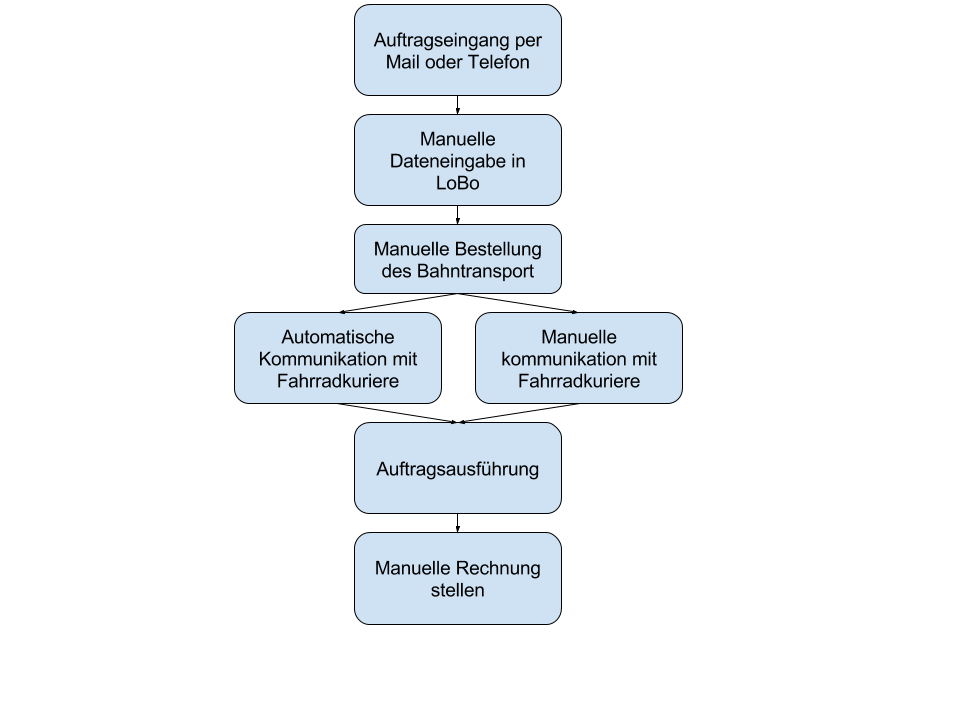
\includegraphics[width=0.88\textwidth]{images/currentProcess.png}
	\caption{Aktueller Prozess für die Erstellung eines Auftrages}
	\label{fig1:currentprocess}
\end{figure}

Bei der manuellen Dateneingabe in LoBo muss der korrekte Bahnhof der Stadt in der eine Lieferung startet und in der sie ankommen soll als zusätzlich zwischen Stopps eingetragen werden. Dadurch weiss der zuständige Fahrradkurier wohin das Paket soll.  Für die Start und Ziel Stadt sind in den meisten Fällen unterschiedliche Fahrradkurier Unternehmen zuständig. Deshalb muss dem Auftrag, sobald der Fahrradkurier der Startstadt das Paket an den Bahnhof gebracht hat, der zuständige Fahrradkurier der Zielstadt zugewiesen werden. Dieser Umstand wird in kauf genommen damit am ende des Auftrages die Abrechnung immer noch korrekt funktioniert. Bevor der Auftrag überhaupt startet muss für das Paket ein Ticket bei der zuständigen Bahngesellschaft bestellt werden. In Deutschland wird der Verkauf von diesen Tickets von time:matters\footnote{time:matters ist eine Tochtergesellschaft von Lufthansa Cargo, welche das Monopol auf das Transportieren von Pakete in Deutschland besitzt \url{http://www.time-matters.com/}} angeboten aber nicht über eine API. Dies wird vom zuständigen Disponenten ausgeführt und dann den beauftragten Fahrradkurieren übermittelt.

\subsection{Software}
Imagine Cargo besitzt 3 LoBo Instanzen. Pro Land gibt es eine Instanz, welche die anderen als Kunden verlinkt hat. Wegen der rechtlichen Problematik, welche zu beginn des Kapitels beschrieben wurde, ist es notwendig dieses umständliche Setup zu benutzten. Imagine Cargo betreibt die Instanzen nicht selber und nutzten die Lösungen direkt als Service.
\textcolor{darkgray}{
  Informationen zur Infrastruktur
}


\section{Marktanalyse}
Beim Versuch einen Überblick über die vorhanden Softwarelösungen auf dem Markt zu bekommen, sind viele Software Lösungen für Speditionen in den Suchresultaten. Viele dieser Software Lösungen sind nur schon unbrauchbar weil sie auf einer klassischen Client-Server Architektur mit ausführbaren Programmen aufbauen. Die wenigen Angebote welche eine webbasierte Benutzeroberfläche anbieten sind aber durch den starken Fokus auf Spedition unbrauchbar. Diese Tools sind besser geeignet eine möglichst effiziente Traveling-Salesman Route zu berechnen als für Kunden welche zum ersten mal versuchen ein Paket mit einem Expresskurier zu verschicken. Die 2 vielversprechendsten Lösungen werden im folgenden kurz vorgestellt.

\subsection{Deliveo}
Deliveo ist eine Software für Kurierdienste und KEP-Dienstleister mit dem Fokus auf motorisierte Fahrzeuge und Fahrräder. Die Benutzeroberfläche von Deliveo macht einen vielversprechenden Eindruck\footnote{Siehe Abbildung \ref{fig1:deliveomask}} und bietet eine grosse Anzahl an Funktionen. Im folgende eine nicht abgeschlossene Liste mit den Funktionen von Deliveo\footnote{ Informationen direkt von der Webseite des Herstellers. \url{http://deliveo.eu/}}.
\begin{itemize}
	\item Das ganze System ist mehrsprachig.
	\item Abrechnung mit dem Kurier(Nachnahme-Preise, Servicepreise und zurückgeholte Dokumente).
	\item Positionsanzeige des Kuriers
	\item Gut entwickeltes API System für die Kommunikation mit anderen Systemen, oder zur Unterstützung der unabhängigen Entwicklungen des Kurierdienstes.
	\item Packet-Betrieb (Aufnahme und Auslieferung) mittels Barcode-Leser mit Smartphone-Kamera
\end{itemize}
Die Benutzeroberfläche welche die Erstellung eines neue Auftrags ermöglicht, scheint den Bedürfnissen welche in Kapitel \ref{sec:personastories} beschrieben sind zu einem grossen Teil gerecht zu werden\footnote{Siehe Abbildung \ref{fig1:deliveonew}}. Das Handhaben macht einen einfachen Eindruck und aus Sicht des Benutzer wirkt es angenehmer als die Eingabemaske von Lobo.

\begin{figure}[ht]
	\centering
  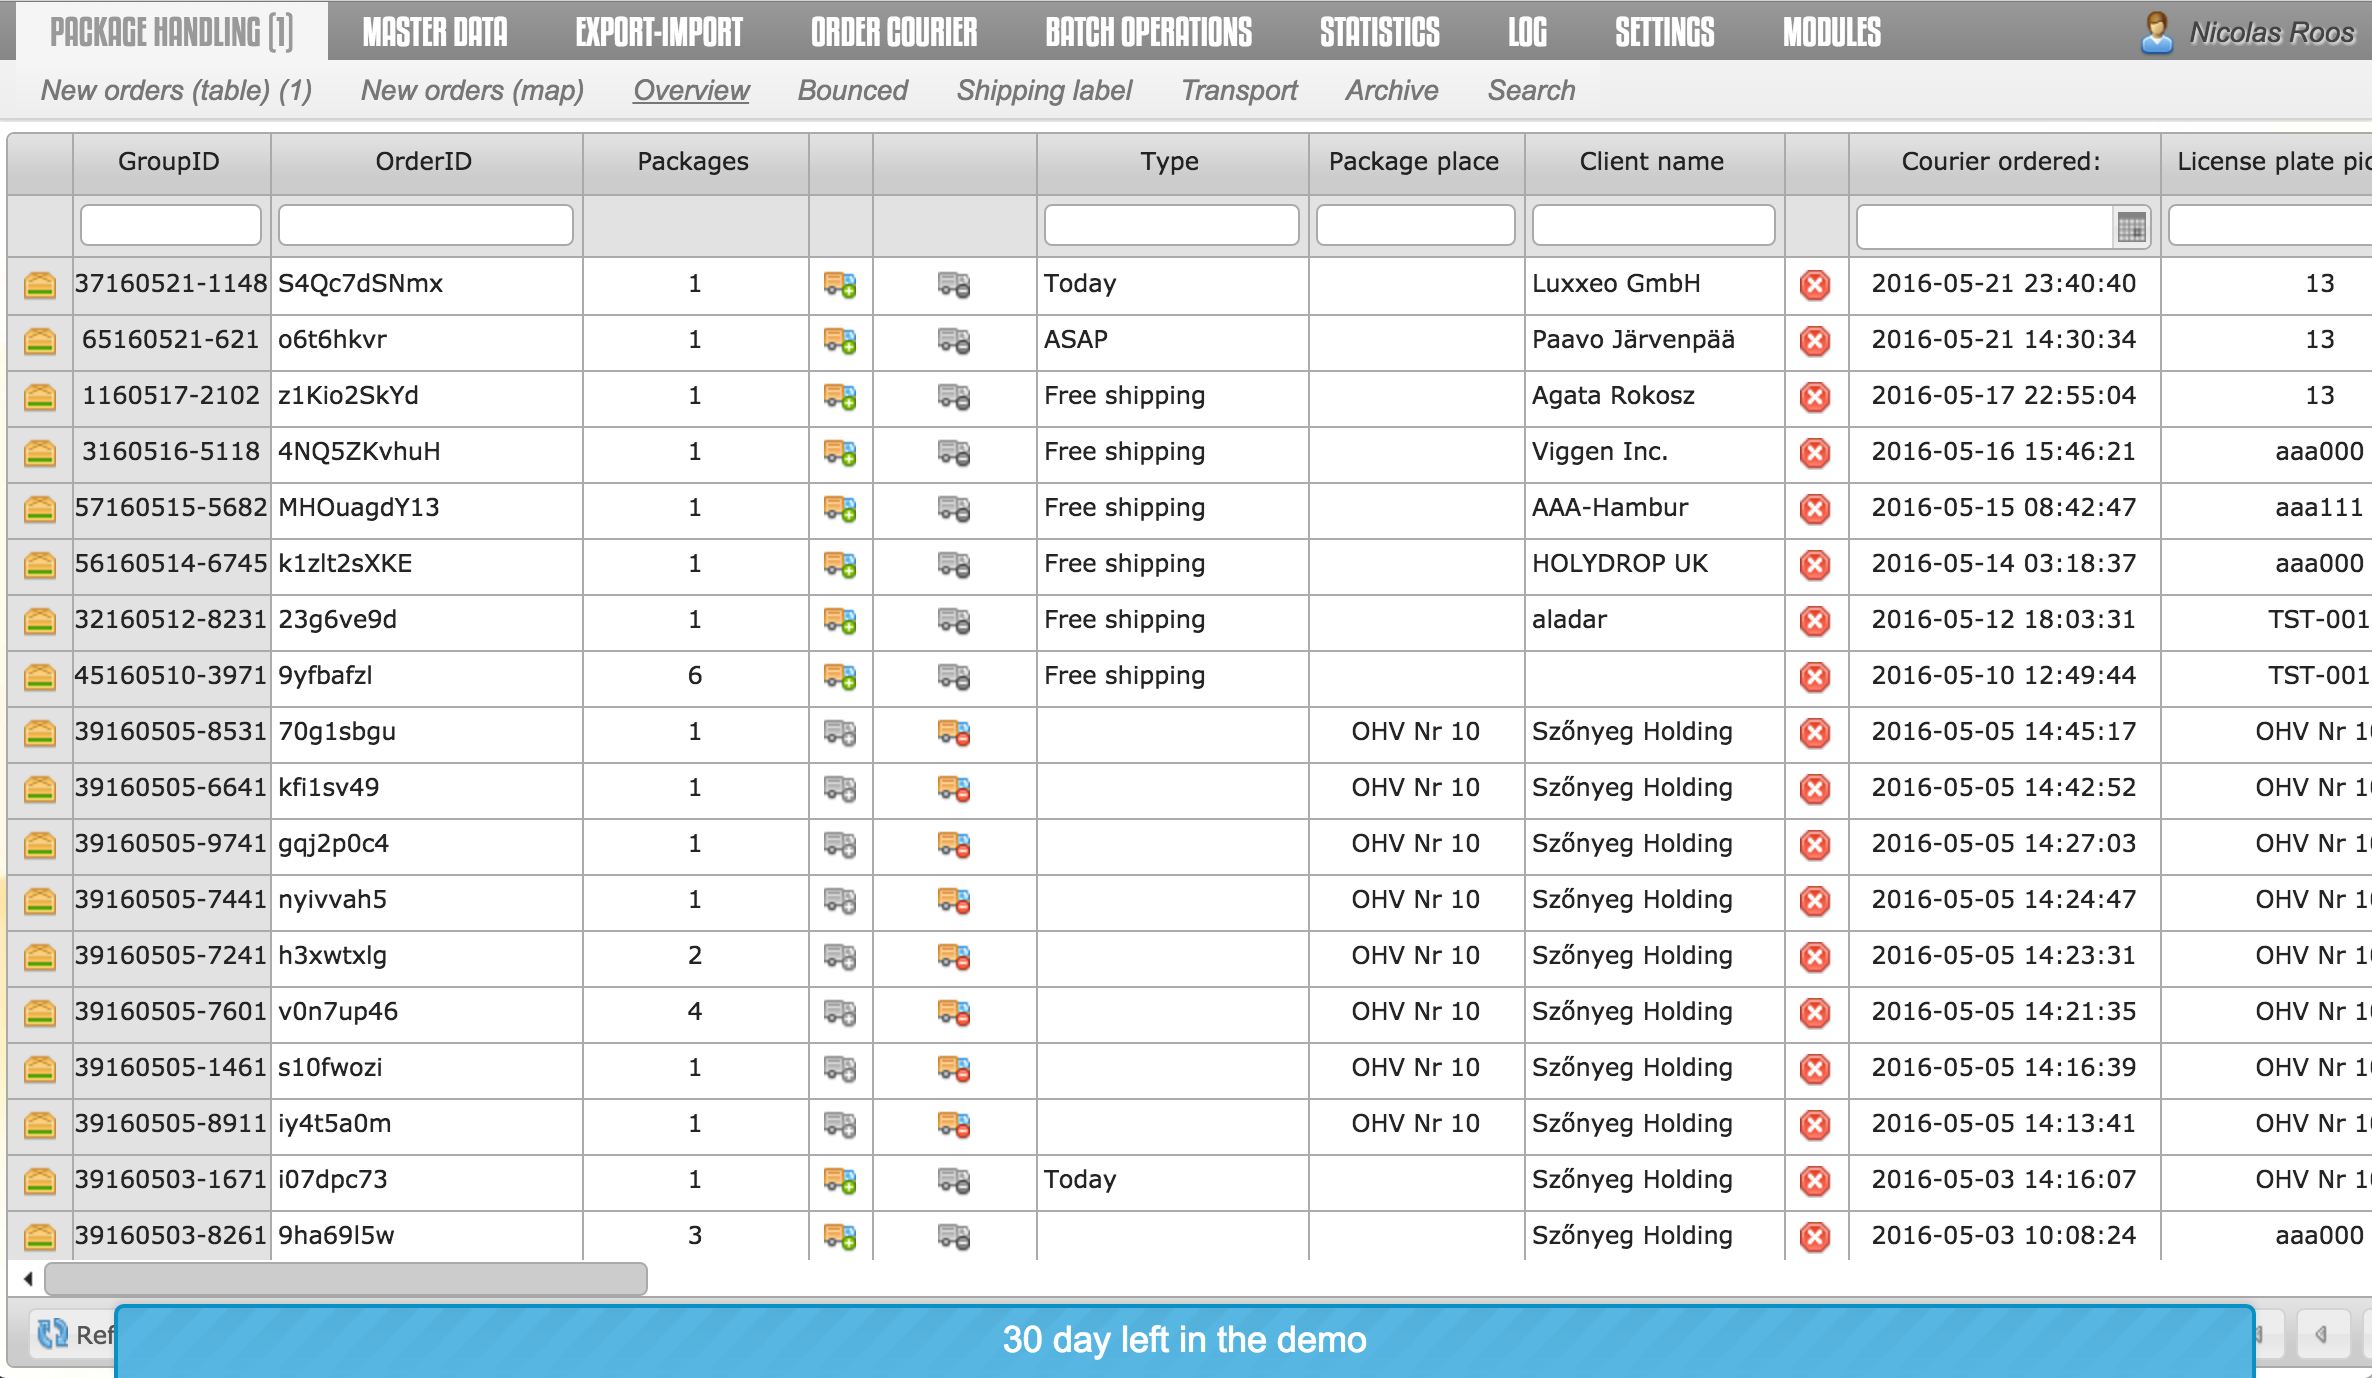
\includegraphics[width=0.88\textwidth]{images/deliveo.png}
	\caption{Auftragsmaske von Deliveo}
	\label{fig1:deliveomask}
\end{figure}

\begin{figure}[ht]
	\centering
  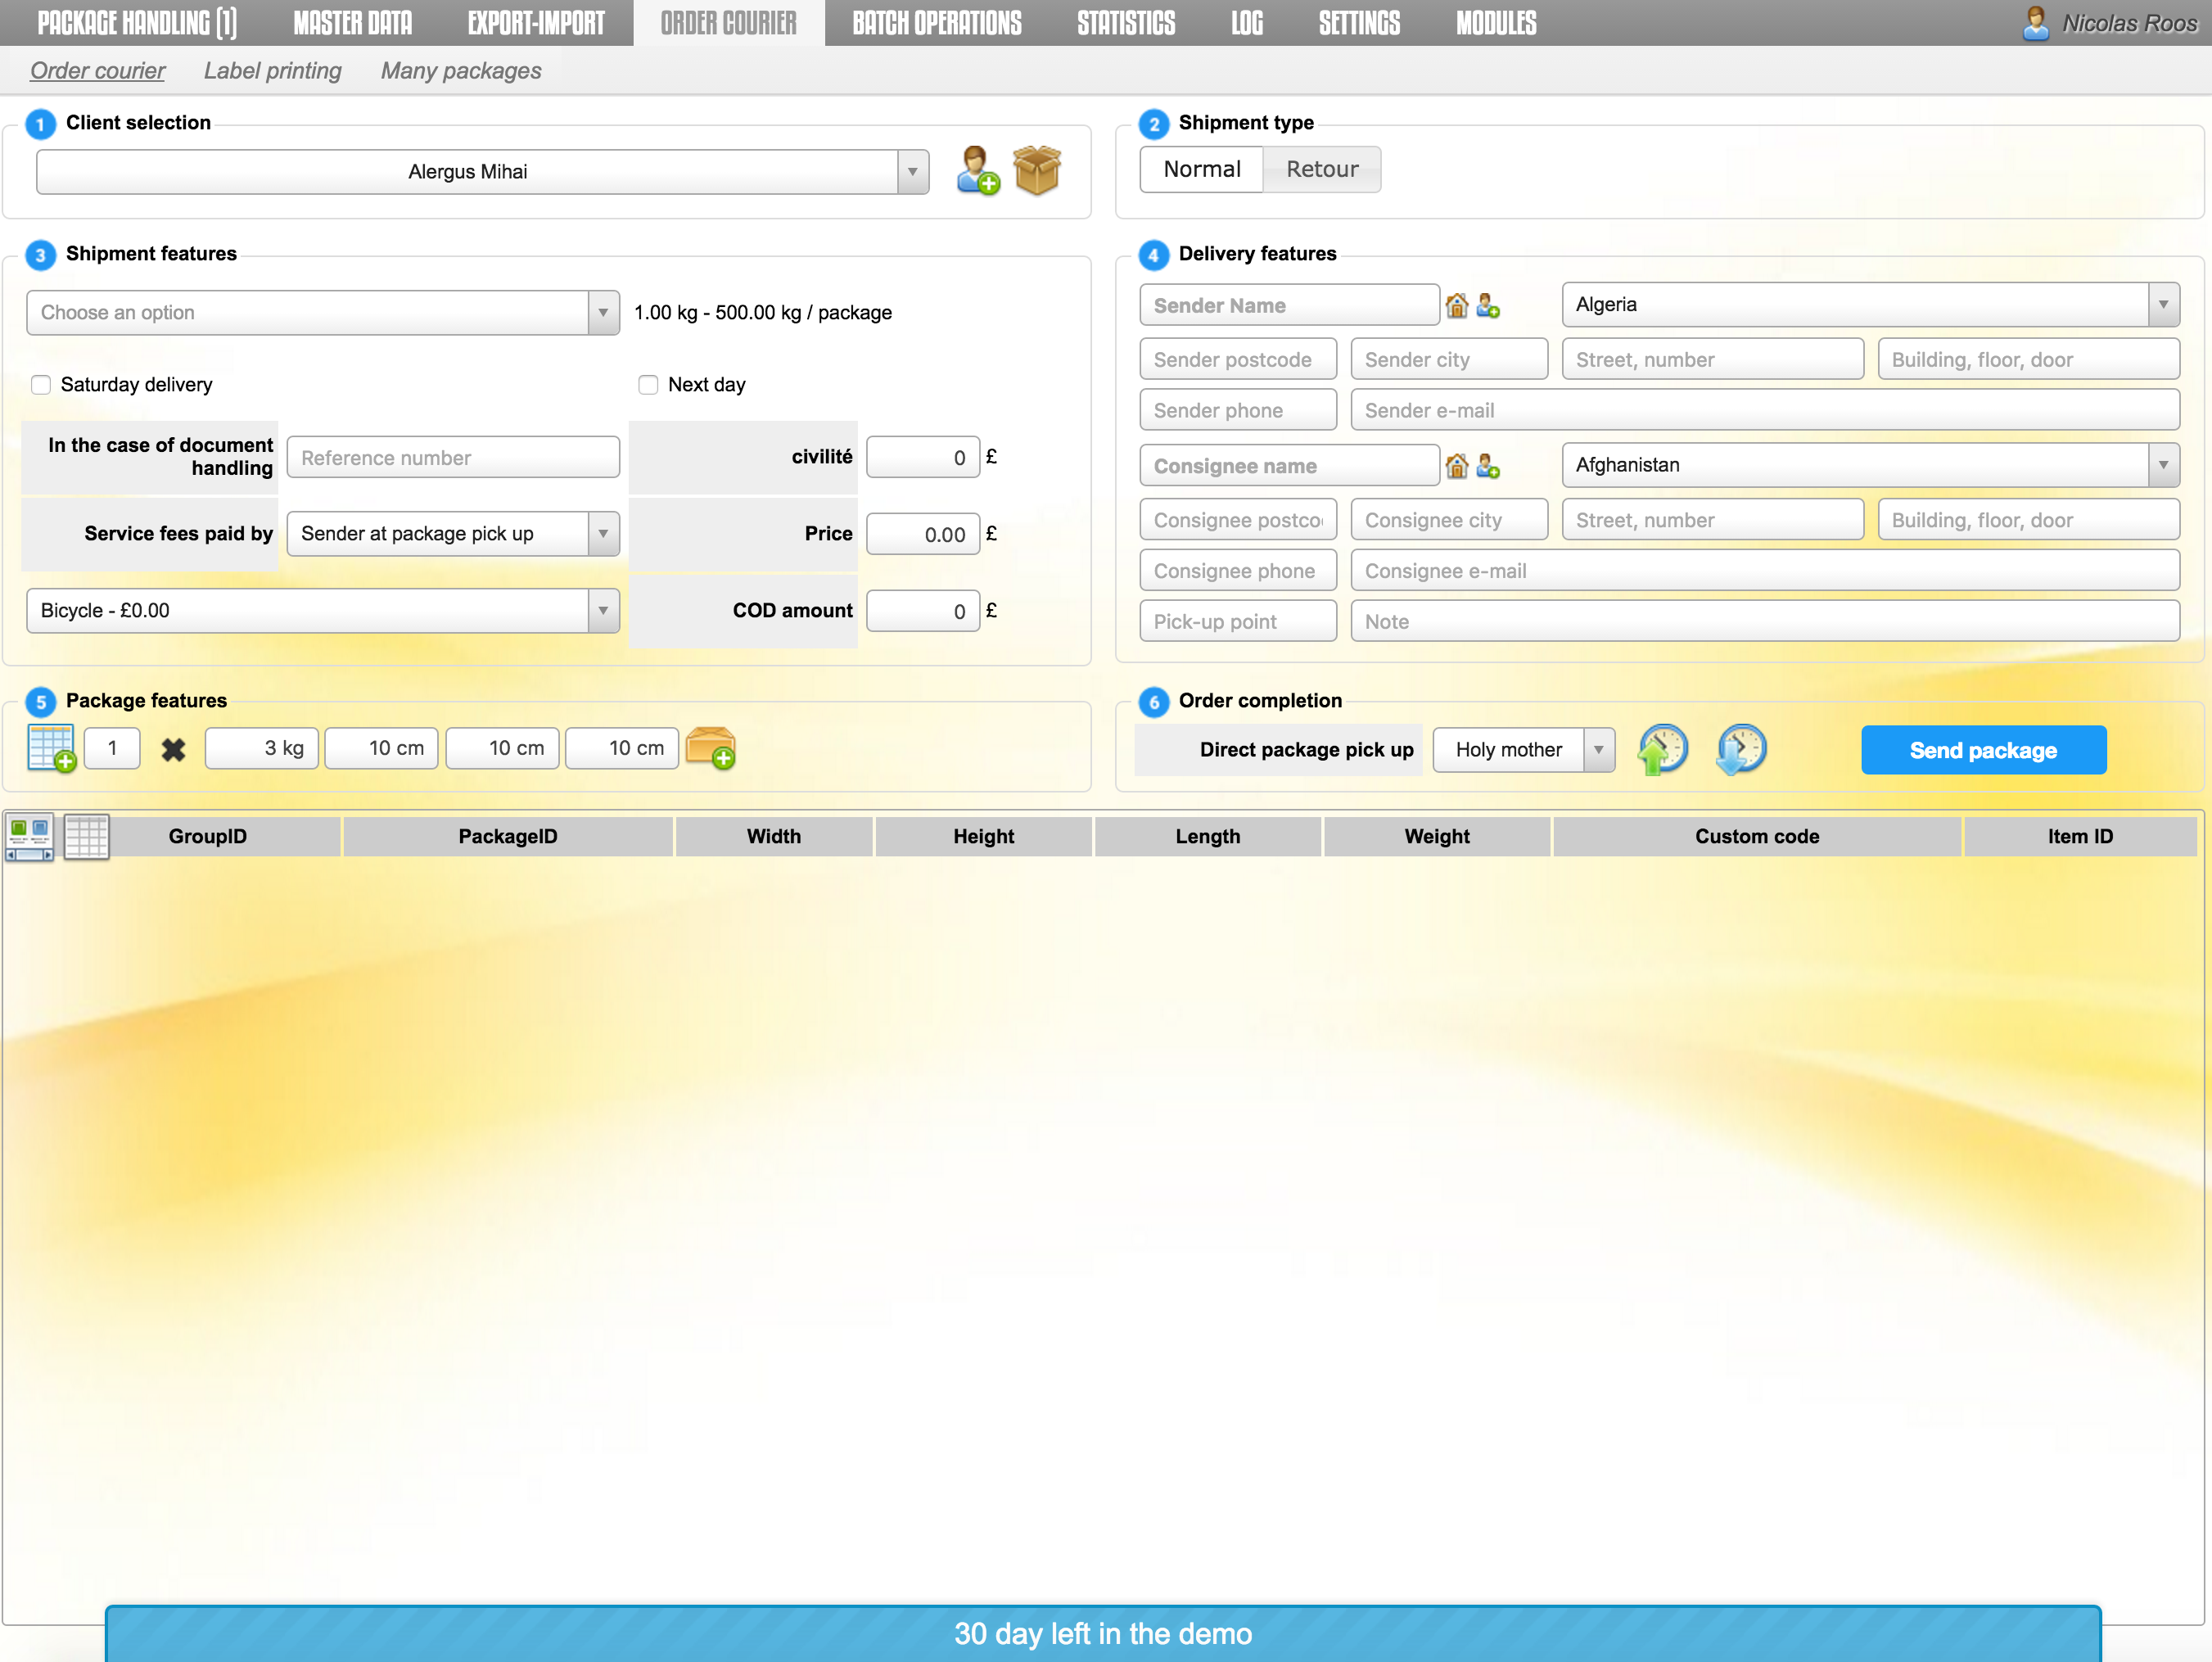
\includegraphics[width=0.88\textwidth]{images/deliveoNew.png}
	\caption{Auftragsmaske für das Erstellen eines neuen Auftrages}
	\label{fig1:deliveonew}
\end{figure}

Deliveo offeriert eine eigene API und obwohl die Dokumentation dieser Schnittstelle in Ungarisch geschrieben ist, ist es möglich damit einen Auftrag zu erstellen.

\subsection{Bamboo Software}
Tested by ImagineCargo. Nicht den Anforderungen standgehalten.

\begin{figure}[ht]
	\centering
  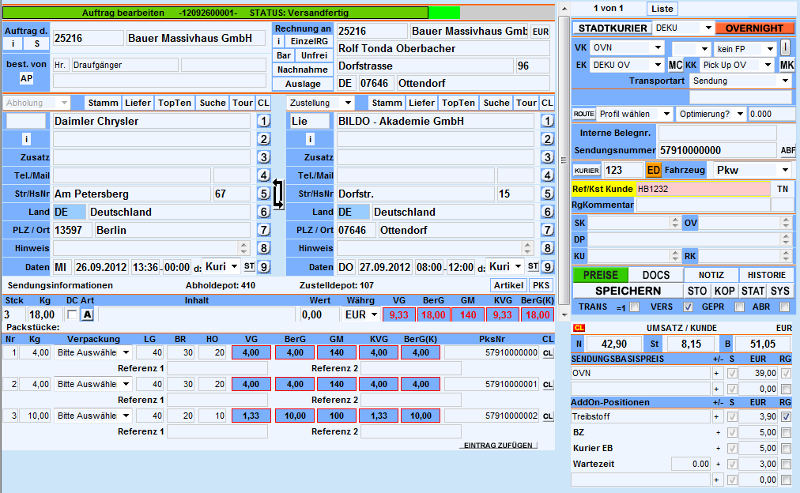
\includegraphics[width=0.88\textwidth]{images/bambooNew.jpg}
	\caption{Auftragsmaske für das Erstellen eines neuen Auftrages}
	\label{fig1:bamboonew}
\end{figure}

\subsection{Schlussfolgerung}
Wegen non functional requirements -> BAAAM.